Zamerajme sa teraz na inštancie, kde vrcholy grafu reprezentujú body v rovine a hrany
vzdialenosti medzi nimi. V prípade obyčajného problému obchodného cestujúceho
existuje PTAS (polynomial time approximation scheme) (\cite{Arora}), t.j. algoritmus, ktorý
pre ľubovoľný aproximačný pomer beží v polynomiálnom čase od veľkosti vstupu.

My v nasledujúcej časti použijeme myšlienky z tohoto algoritmu a ukážeme PTAS pre
problém dvoch obchodných cestujúcich.

Hlavnou myšlienkou algoritmu je pomocou techniky rozdeľuj a panuj vybudovať nad vstupom
randomizovaný quad-tree. Následne ukážeme, že pre $(1 + 1/c)$-aproximačný algoritmus stačí, aby
TSP-cesty pretínali hrany delenia iba $O(c)$ krát. Navyše tieto prieniky sa môžu
udiať iba v niektorých špeciálnych bodoch.

\section{Rekurzívne delenie}

%Rovinu v ktorej ležia vstupné body budeme rekurzívne deliť na menšie časti.
%Najprv rovinu rozdelíme vodorovnou a zvislou čiarou na štyri časti, každú z nich na ďalšie štyri, ...
%Takto by sme dostali tzv. quadtree. Na správnu fukčnosť algoritmu potrebujeme ale tzv.
%posunutý quadtree, kde deliace čiary neprechádzajú stredom, ale sú vyberané náhodne.
%

Pre začiatok predpokladajme, že všetky body majú celočíselné súradnice a vzdialenosť
medzi nimi je aspoň $8$. Neskôr ukážeme, že každý vstup vieme takto upraviť a ak budeme mať PTAS
pre upravený vstup, tak budeme mať PTAS aj pre pôvodný vstup.

Nech všetky body ležia vo vnútri štvorca $S$ so stranou $L$, ktorého ľavý dolný roh
má súradnice $[0,0]$. Navyše bez ujmy na všeobecnosti nech je $L$ mocnina dvojky.

{\bf Rekurzívnym delením} štvorca $S$ nazývame jeho rekurzívne delenie na menšie štvorce tak, že
každy štvorec rozdelíme {\bf deliacimi čiarami} na štyri rovnaké štvorce.
Deliť prestaneme, keď je strana štvorca $\leq 1$. Toto delenie predstavuje
$4$-árny strom, kde synovia každé ho štvorca sú štyri menšie štvorce. Hĺbka takéhoto stromu je
najviac $O(\lg L)$. 
Štvorcom delenia intuitívne priradíme úrovne. Štvorec $S$ má úroveň $0$, jeho synovia úroveň $1$,
atď. Deliaca čiara má úroveň $i$ vtedy, keď obsahuje hranu nejakého štvorca úrovne $i$, ale žiadneho
úrovne väčšej ako $i$.

{\bf Quadtree} definujeme podobne 
až na to, že rekurzívne delenie skončí vtedy, keď v danom štvorci je najviac jeden bod. Keďže každý
list quadtree obsahuje bod zo vstupu, alebo je súrodenec takého listu, tak quadtree má maximálne
$O(n)$ listov a teda dokopy najviac $O(n \lg L)$ štvorcov.

\smallskip

Teraz popíšeme posunuté delenie. Nech $a, b$ sú celé čísla a platí $0 \leq a, b < L$.
$(a,b)$-posunutie rekurzívneho delenia definujeme tak, že $x$-, $y-$ súradnice každej deliacej čiary
zvýšime o $a$ resp. $b$ a následne spočítame ich zvyšok po delení číslom $L$ (vstupnými bodmi
nehýbeme). Takisto posunieme aj okrajové čiary štvorca (začnú tvoriť deliace čiary). Pôvodný štvorec
pokladáme za zacyklený, teda okrajové oblasti pri posunutom delení tvoria súvislú oblasť ako na
obrázku \ref{fig:quadtree}.

Z posunutého rekurzívneho delenia vieme dodefinovať quadtree s posunom tak, že nebudeme deliť
štvorce, ktoré obsahujú najviac jeden bod.

\section{Portály a $(m,r)$-ľahké cesty}

\begin{figure}[h]
\centering
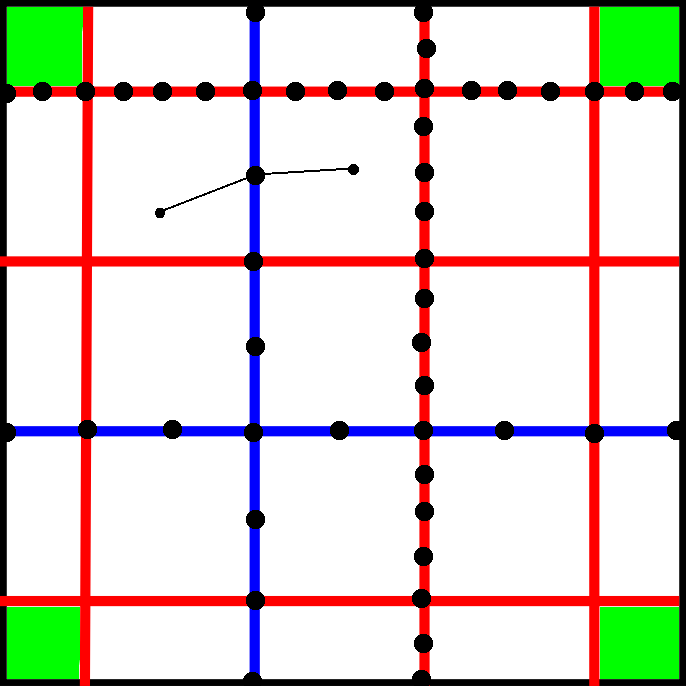
\includegraphics{img/quadtree.png}
\caption{Posunuté rekurzívne delenie a portály}
\label{fig:quadtree}
\end{figure}

Nás algoritmus dovolí TSP-cestám pretínať čiary delenia iba v niekoľkých
predpísaných bodoch, tzv. {\bf portáloch}. Toto je na prvý pohľad trochu kontraintuitívne.
My ale dovolíme cestujúcim cestovať medzi bodmi po ľubovoľnej čiare, teda nie nutne najkratšej
ceste medzi dvoma bodmi (viď. obr. \ref{fig:quadtree}). Stále ale zachovávame disjuktnosť ciest, t.j. keď
jeden cestujúci ide z vrchola $x$ do vrcholu $y$, tak druhý nemôže ísť z $x$ do $y$ ani z $y$ do
$x$ (nech ide ľubovoľne zakrivenou cestou). 

\begin{definicia}
Nech $m$ je párne kladné celé číslo. $m$-regulárna množina portálov pre posunuté rekurzívne
delenie je množina bodov taká, že každá deliacia čiara úrovne $i$ obsahuje portály vo
vzdialenostiach $\frac{L}{m2^i}$. 
\end{definicia}


\begin{definicia}
TSP-cesta sa nazýva $(m,r)$-ľahká ak pretína čiary rekurzívneho delenia iba v $m$-regulárnej
množine portálov a navyše každú hranu štvorca pretína najviac $r$-krát.
\end{definicia}

Teraz sformulujeme hlavnú vetu, ktorá dokazuje koreknosť nášho algoritmu.

\begin{veta}
Nech $c > 0$ je ľubovoľná konštanta. Nech je každá nenulová vzdialenosť vo vstupe aspoň $8$ a nech všetky
body ležia vo vnútri štvorca so stranou $L$. Nech $0 \leq a, b < L$ sú vybrané náhodne. Potom s
pravdepodobnosťou aspoň $1/2$ existujú dve disjuktné $(m,r)$-ľahké TSP-cesty, ktorých dĺžka je maximálne $(1 +
1/c)$-násobok optimálnej dĺžky, pričom $m = O(c \lg L)$, $r = O(c)$.
\end{veta}

Dôkaz tejto vety uvedieme neskôr. 
Najprv sa pozrime na hľadanie najkratších $(m, r)$-ľahkých ciest.

\section{Popis algoritmu}

Ako sme už spomínali, algoritmus predpokladá, že vstupná inštancia je "slušná", t.j.:
\begin{itemize}
\item Body majú celočíselné súradnice.
\item Nenulová vzdialenosť bodov je aspoň 8.
\item Najväčšia vzdialenosť bodov je $O(n)$.
\end{itemize}

Vstupnú inštanciu upravíme na inštanciu, ktorá spĺňa tieto podmienky nasledovne:
Nech $L_0$ je dĺžka strany štvorca v ktorom leží vstupná inštancia a $d$ je dĺžka optimálneho
riešenia. Navyše platí $L_0 \leq d$. V štvorci vyrobíme mriežku s veľkosťou bunky 
$\frac{d}{8nc}$ a každy bod presunieme do najbližšieho mrežového bodu.
Dĺžka jednej kružnice sa zmení maximálne o $\frac{2nL_0}{8nc} < \frac{d}{4c}$.
Dĺžka dvoch kružníc sa zmení maximálne o $\frac{d}{2c}$. Teraz zmenšíme všetky vzdialenosť
$\frac{L_0}{64nc}$ krát. Teda všetky súradnice budú celočíselné a minimálna nenulová vzdialenosť bodov
bude aspoň $8$. Navyše dĺžka strany štvorca, v ktorom ležia body, bude $O(nc)$, čo je $O(n)$, keďže
$c$ je konštanta.
Po takejto transformácii, ale namiesto $1 + 1/c$ aproximácie musíme hľadať $1 + 1/2c$ aproximáciu,
ale to nám nevadí, keďže $c$ môže byť ľubovoľná kladná konštanta.

\bigskip

V nasledujúcom kroku zvolíme hodnoty $a, b$ -- posuny quad-tree. Môžeme ich zvoliť náhodne
a uspokojiť sa s tým, že máme iba pravdepodnostný algoritmus, alebo môžeme postupne vyskúšať všetky
hodnoty za cenu vyššej časovej zložitosti o faktor $O(n^2)$. Pre zvyšok tejto kapitoly budeme
predpokladať, že $a, b$ volíme náhodne. Teraz môžeme skonštruovať posunutý quad-tree. 
Keďže po predchádzajúcom kroku máme $L = O(n)$ a hĺbka quad-tree je teda najviac $O(\lg n)$, potom
počet štvorcov v quad-tree je $O(n \lg n)$ (lebo máme maximálne $n$ listov). Tento quadtree vieme
pomerne jednoducho skonštruovať v čase $O(n \lg n)$.

Teraz ideme nájsť v skonštruovanom posunutom quad-tree nájsť najlacnejšie $(m,r)$-ľahké disjuktné
TSP cesty. Využijeme techniku dynamického programovania.

Zoberme si štvorec $S$ z quad-tree a optimálne $(m,r)$-ľahké TSP cesty. Prvá z nich pretína hranicu
štvorca $S$ postupne v bodoch $a_1, a_2, \dots, a_{2p}$, kde $2p \leq 4r$ a druhá v bodoch $b_1, b_2,
\dots, b_{2q}$, kde $2q \leq 4r$. 

Časti TSP ciest vo vnútri $S$ je postupnosť ciest, ktoré majú konce v bodoch $a_{2i - 1}, a_{2i}$,
resp. $b_{2j - 1}, b_{2j}$, pre $i = 1, 2, \dots, p$, resp. $j = 1, 2, \dots q$.
Tieto cesty navyše prechádzajú všetkými bodmi vo vnútri $S$ a ich zjednotenie je $(m,r)$-ľahké.
Navyše sú tieto cesty disjuktné, t.j. neexistujú dva vrcholy $v_i$, $v_j$ vo vnútri $S$ také, že 
v obidvoch postupnostiach sú $v_i$ a $v_j$ spojené.
Ešte si všimnime vrcholy, ktoré nasledujú na cestách po jednotlivých prienikoch (keď pokračujeme po
ceste od prieniku smerom dovnútra štvorca).
Postupne ich označme pre prvú cestu ako $v^a_1, v^a_2, \dots, v^a_{2p}$ a pre druhú cestu ako
$v^b_1, v^b_2, \dots, v^b_{2q}$. Tieto vrcholy nemusia byť nutne vrcholy vo vnútri $S$, keďže časť
cesty môže prechádzať cez štvorec $S$, ale nemusí prechádzať cez žiadny vrchol.

Keďže máme optimálnu $(m,r)$-ľahkú cestu, tak aj postupnosť ciest uvedená vyššie je optimálna, t.j.
najlacnejšia taká, že jednotlivé cesty majú konce v zadaných bodoch $a_1, a_2, \dots, a_{2p}$, resp. $b_1, b_2,
\dots, b_{2q}$, najbližšie vrcholy ku koncom sú $v^a_1, v^a_2, \dots, v^a_{2p}$, resp.
$v^b_1, v^b_2, \dots, v^b_{2q}$ a tieto cesty prechádzajú všetkými bodmi vo vnútri $S$ a zároveň sú
disjuktné.

Teraz môžeme definovať vhodný podproblém pre dynamické programovanie. Jeho vstupmi budú:
\begin{itemize}
\item Štvorec $S$ z posunutého quad-tree.
\item Postupnosti portálov, ktoré majú cesty pretínať: $a_1, a_2, \dots, a_{2p}$, $b_1, b_2, \dots,
b_{2q}$.
\item Postupnosti vrcholov, do ktorých pôjdu cesty za portálmi: $v^a_1, v^a_2, \dots, v^a_{2p}$,.
$v^b_1, v^b_2, \dots, v^b_{2q}$.
\end{itemize}

Jeho výstupom je postupnosť ciest definovaná vyššie.

Predtým než ukážeme ako tento podproblém riešiť spočítame počet rôznych podproblémov.
Ako sme spomínali máme $O(n \lg n)$ štvorcov. Rôznych postupnosti portálov bude $O(m^{O(r)})$.
Rôznych postupnosti vrcholov bude $O(n^{O(r)})$. Keďže $r = O(c)$, tak stále
máme PTAS. Neskôr ukážeme ako zmenšiť člen $O(n^{O(r)})$ na člen $O(n)$.

Podproblémy vieme riešiť nasledovne. Pokiaľ obsahuje štvorec iba jeden vrchol vieme v čase $O(r)$. vyskúšať všetky
možné priradenia. Zobereme si teraz štvorec $S$, ktorý má synov $S_1, S_2, S_3, S_4$. Pre jeho synov
už máme vyriešené všetky podproblémy. Chceme teraz nájsť najlacnejšie $(m, r)$-ľahké cesty pre
štvorec $S$. Preskúšame všetky možnosti akoby cesty mohli prechádzať hranami štvorcov $S_1, S_2,
S_3, S_4$. To obnáša vybrať poradie prechodu portálmi a vrcholy, ktorými cesta bude prechádzať po
prechode portálom. Ešte potrebujeme skontrolovať disjukntosť ciest. Medzi vrcholmi vrámci štvorcov
$S_1, S_2, S_3, S_3$ máme disjuknosť zaručenú. Treba ešte zaručiť aj disjuktnosť ak cesta prechádza
medzi vrcholmi z rôznych štvorcov. To vieme zaručiť pomocou toho, že sa pozrieme aké vrcholy
nasledujú za portálmi a nepovolíme tie možnosti, v ktorých sú spojené rovnaké dvojice vrcholov v
oboch TSP cestách. Časová zložitosť tohoto kroku je najviac $O(n^{O(r)} m^{O(r)})$.

Celkový čas tohoto algoritmu je $O(n^{O(r)} m^{O(r)})$, čo je $O(n^{O(c)})$.

\section{Dôkaz hlavnej vety}

Pri dôkaze hlavnej vety využijeme dve pomocné lemy. Prvou z nich je tzv. "Patching lema".
Pre problém obchodného cestujúceho je jej znenie nasledovné:

\begin{lema}[Patching lema]
Existuje konštanta $g > 0$ taká, že platí nasledovné: Nech $S$ je úsečka dĺžky $s$ a $\pi$ je
uzavretá cesta, ktorá pretína $S$ aspoň $3$-krát. Potom existuje množina podúsečiek $S$ s dĺžkou najviac
$gs$, ktorých pridaním do $\pi$ dostaneme cestu $\pi^{'}$, ktorá pretína $S$ najviac $2$-krát.
\end{lema}

Dôkaz tejto lemy sa dá nájsť v \cite{Arora}. My ho tu stručne zhrnieme.

\begin{dokaz}
Predpokladajeme, že $\pi$ pretína $S$ práve $t$ krát v bodoch $M_1, M_2, \dots, M_t$ -- body
označíme v poradí v akom sa vyskytujú na úsečke $S$.
Cestu $\pi$ v týchto bodoch rozsekneme na $t$ častí $P_1, P_2, \dots, P_t$. Z každého bodu $M_i$
si pripravíme dve kópie -- $M_i^{'}$ a $M_i^{''}$, každú kópiu umiestnime na jednu stranu $S$.
Nech $J$ je multimnožina úsečiek, ktorá obsahuje nasledovné:
\begin{itemize}
\item Najlacnejšiu kružnicu, ktorá prechádza cez body $M_1, M_2, \dots, M_t$.
\item Najlacnejšie perfektné párenie medzi bodmi $M_1, M_2, \dots, M_{2k}$, kde $2k$ je najväčšie
párne číslo menšie ako $t$. 
\end{itemize}

Množina $J$ má dĺžku najviac $3s$. Množinu $J$ opäť zoberieme v dvoch kópiách -- $J^{'}$, $J^{''}$ a pridáme ju k ceste $\pi$.
Ešte navyše ak je $t$ nepárne, tak spojíme body $M_{2k+1}^{'}$ a $M_{2k+1}^{''}$ a ak je $t$ párne,
tak spojíme body $M_{2k+1}^{'}$ a $M_{2k+1}^{''}$ a body $M_{2k+2}^{'}$ a $M_{2k+2}^{''}$.
Spolu cesty $P_1, P_2, \dots, P_t$ a pridané úseky tvoria $4$-regulárny graf na vrcholoch
$\{M_1^{'}, \dots, M_t^{'}\} \cup \{M_1^{''}, \dots, M_t^{''}\}$. Eulerovský ťah na tomto grafe
prechádza všetkými cestami $P_1, \dots, P_t$ a navyše pretína $S$ najviac dvakrát. Navyše
súčet všetkých pridaných úsečiek je najviac $6s$. A teda sme dokázali túto vetu pre $g = 6$.
\end{dokaz}

My potrebujeme túto lemu zovšeobecniť pre dvoch obchodných cestujúcich.

\begin{lema}
Existuje konštanta $g > 0$ taká, že platí nasledovné: Nech $S$ je úsečka dĺžky $s$ a $\pi$ je
uzavretá cesta, ktorá pretína $S$ aspoň $20$-krát. Nech $\pi_2$ je cesta disjuktná s $\pi$.
Potom existuje množina podúsečiek $S$ s dĺžkou najviac
$gs$, ktorých pridaním do $\pi$ dostaneme cestu $\pi^{'}$, ktorá pretína $S$ najviac $20$-krát a
zároveň nepretína cestu $\pi_2$.
\end{lema}

\begin{dokaz}
Vďaka patching leme vieme cestu $\pi$ previesť na cestu $\pi^{'}$, ktorá pretína $S$ najviac
dvakrát. Predpokladajme, že $\pi^{'}$ bola zostrojená pomocou predchádzajúceho dôkazu a teda vedie
cez body $M_1^{'}, \dots, M_t^{'}, M_1^{''}, \dots, M_t^{''}$. Táto cesta môže ale zdieľať niektoré
hrany s cestou $\pi_2$. Teda môže existovať niekoľko dvojíc bodov $(x, y)$ takých, ktoré sú spojené
aj v $\pi$ aj v $\pi_2$. Týchto dvojíc je najviac $2t$, keďže najviac $2t$ bodom sme zmenili suseda. 

Zakázanou dvojicou budume nazývať dvojicu bodov $(x, y)$ takú, že $x$ a $y$ sú susedné na
ceste $\pi_2$. Každý vrchol sa teda vyskytuje práve v dvoch zakázaných dvojiciach.

Našim cieľom je upraviť cestu $\pi^{'}$ tak, aby neobsahovala ani jednu zakázanú dvojicu.
Zakázané dvojice budeme odstránovať postupne.

Nech $(x,y)$ je zakázaná dvojica, ktorá sa vyskytuje v $\pi^{'}$. Rozlišujeme niekoľko prípadov
(všetky prípady majú obdobu pre druhú stranu úsečky $S$).
\begin{enumerate}
\item Cesta $\pi^{'}$ od $x$ smerom k $y$ najprv prechádza bodmi $M_i^{'}$ a $M_{i+1}^{'}$ (resp.
$M_{i-1}^{'}$.
\item Cesta $\pi^{'}$ od $x$ smerom k $y$ najprv prechádza bodmi $M_t^{'}$ a $M_{1}^{'}$ (alebo
opačne).
\item Cesta $\pi^{'}$ od $x$ smerom k $y$ najprv prechádza bodmi $M_i^{'}$ a $M_i^{''}$ (alebo
opačne), kde $i = t$, alebo $i = t-1$.
\end{enumerate}

Myšlienka odstránenia zakázanej dvojice bude nasledovná. V blízkosti $M_i^{'}$ (resp. $M_t^{'}$)
nájdeme úsečku medzi bodmi $M_j^{'}$, $M_j^{'}$, cez ktorú cesta $\pi_{'}$ spája vrcholy $u, v$
a dvojice $(x,u), (x,v), (y,u), (y,v)$ nie sú zakázané. Potom prehodíme úsečky tak, že spojíme
vrcholy $x$ a $v$ a vrcholy $y$ a $u$ (resp. opačne), tak aby sme opäť dostali uzavretú cestu.
Teraz už len potrebujeme dokázať, že úsečka s požadovanou vlastnosťou existuje.

Ukážeme to pre prvý prípad, ostatné sú obdobné. 
Nech $(x, a)$ a $(y, b)$ sú zakázané dvojice pre body $x, y$ iné ako $(x,y)$. 
Zoberme si postupne najbližších susedov $M_i^{'}$. Pre suseda $M^{'}_j$ sa pozrime na najbližší vrchol na
ceste $P_j$ (resp. $P_{j+1}$), ktorá tam končí (predpokladáme, že táto cesta má aspoň jeden vrchol, ináč by sme počet
pretnutí úsečky vedeli znížiť iným spôsobom). Tento vrchol označme $z$. Bod $M^{'}_j$ leží teda
medzi vrcholom $z$ a nejakým iným vrcholom $z^{'}$.  

Našim cieľom je nájsť $M_j^{'}$ také, že $z$ a $z^{'}$ sú iné ako $x, y, a, b$. Každý vrchol sa môže
vyskytnúť ako najbližší vrchol dvakrát. Navyše sa každý z nich môže dva krát vyskytnúť ako sused
najbližšieho vrchola. To znamená, že potrebujeme prešetriť aspoň 17 bodov $M_j^{'}$.
Aby sme sa vyhli zavádzaniu ďalších pretnutí úsečky $S$ nebudeme sa pozerať na body $M_t^{'}$ a
$M_{t-1}^{'}$. To znamená, že ak máme $20$ rôznych bodov pretnutia, tak určite nájdeme nejaký vhodný bod.

Úplne rovnakým spôsobom vieme vyriešiť druhý prípad. V treťom prípade je jediným problémom to, že
nám vznikne navyše niekoľko pretnutí úsečky $S$, ale pre jedno odstránenie zakázanej dvojice vznikne
maximálne jedno nové pretnutie. A takého zakázane dvojice búdu najviac $4$. 

Takýmto spôsobom odstránime všetky zakázané dvojice. Ešte treba ukázať, že nezvýšime dĺžku cesty
o viac ako konštatný násobok $s$. Keďže každý bod pripojíme v najhoršom prípade k $17$-tému
najbližšiemu bodu, tak celkové predĺženie bude najviac $34s$ (lebo môžeme prepájať body na oboch
stranách). 
\end{dokaz}

Zvyšok dôkazu je rovnaký ako v \cite{Arora} až na zmenu niekoľkých konštánt.
TODO: možno ho tu napísať

\section{Rýchlejší algoritmus}

Počet stavou v doteraz popísanom algoritme najviac dvíhala nutnosť pamätať si, ktorý vrchol
nasleduje za ktorým prechodom. Túto informáciu sme si pamätali preto, aby sme zabezpečili
disjuktnosť ciest vtedy keď spájame informácie z jednotlivých synov štvorca v quad-tree.

Disjuktnosť vieme zabezpečiť aj s menším počtom stavov.
Stačí nám vedieť, že či za dvoma prechodmi portálmi leží rovnaký vrchol.
Keď cesta pretne štvorec v portáli $a_i$, tak máme nasledovné možnosti:
\begin{itemize}
\item Cesta prechádza štvorcom bez toho, aby prešla cez nejaký vrchol.
\item Cesta vojde do štvorca a prvý vrchol cez ktorý prejde je vrchol $v_i$.
V tomto prípade môže existovať žiaden, jeden alebo dva portály -- $b_{i_1}, b_{i_2}$ --
pre druhú cestu také, že druhá cesta po prejdení týmito portálmi vojde
do vrchola $v_i$.
\end{itemize}

Pri spájaní podproblémov potom vieme overiť disjuktnosť práve na základe tejto informácie.

Vstupy podproblému teda budú:
\begin{itemize}
\item Štvorec $S$ z posunutého quad-tree.
\item Postupnosti portálov, ktoré majú cesty pretínať: $a_1, a_2, \dots, a_{2p}$, $b_1, b_2, \dots, b_{2q}$.
\item Pre každé pretnutie portálu informácia o rovnakom vrchole za portálom, tak ako je uvedené
vyššie.
\end{itemize}

Keď spočítame počet podproblémov, tak dostaneme. $O(n \lg n)$ štvorcov, $O(m^{O(r)})$
postupnosti portálov a $O(r^{O(r)})$ možností ako môžu mať portály spoločné vrcholy.
Celkovo máme teda aj časovú zložitosť $O(n (\lg n)^{O(c)} c^{O(c)})$. 
